
\subsection{Reaction hierarchy}

\begin{figure}[!h]
  \centering
  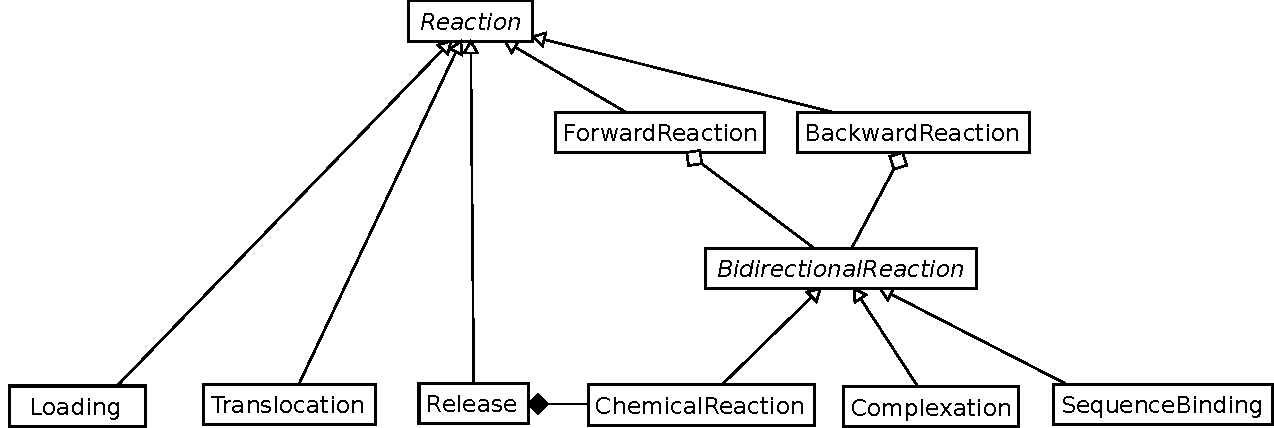
\includegraphics[width=\linewidth]{reaction_uml}
  \caption{UML diagram of \texttt{Reaction} hierarchy.}
  \label{fig:reaction_uml}
\end{figure}

This section gives a quick overview of the reaction hierarchy~\reffigp{fig:reaction_uml}. More details about how reactions are implemented can be found later.

\subsubsection{Reaction}

\begin{figure}[!h]
  \centering
  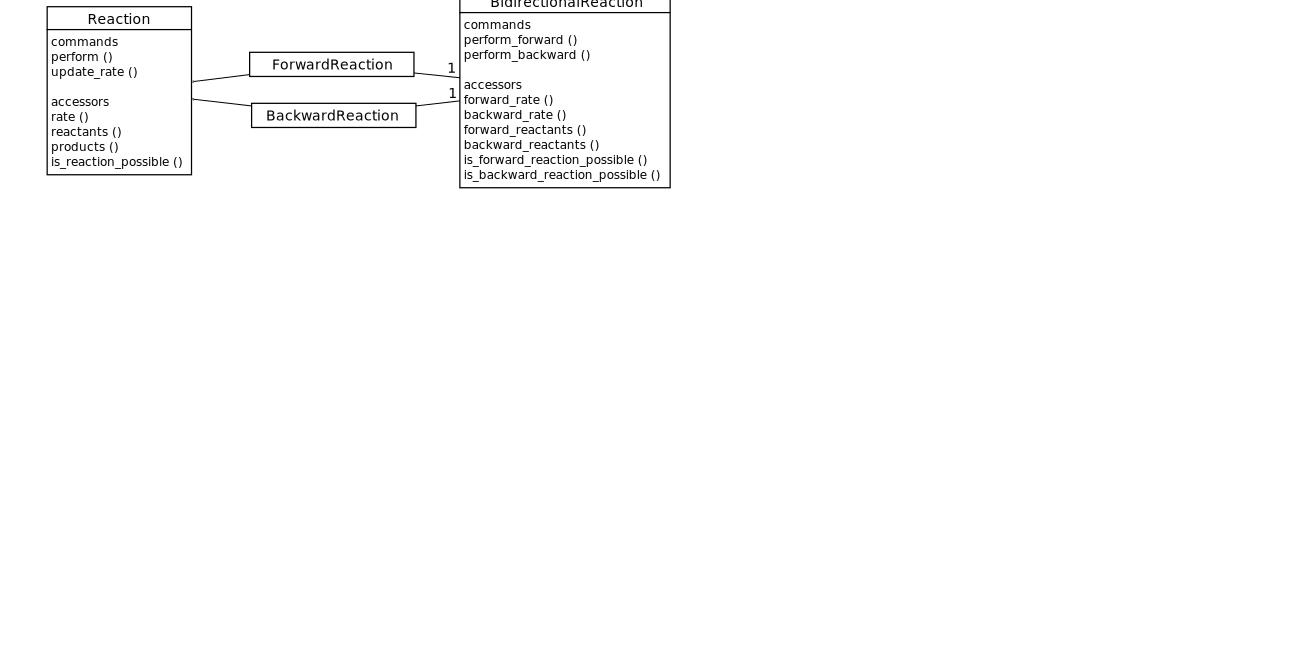
\includegraphics[width=0.8\linewidth]{reaction}
  \caption{\texttt{Reaction} and \texttt{BidirectionalReaction} classes.}
  \label{fig:reaction}
\end{figure}

There are two abstract classes used to define reactions: \texttt{Reaction} for one-way reactions and \texttt{BidirectionalReaction} for reversible reactions. Two adapter classes \texttt{ForwardReaction} and \texttt{BackwardReaction} split reversible reactions in two one-way reactions\reffigp{fig:reaction}. In the end, the solver only handles one-way reactions. A reaction can necessarily be performed, its rate updated and accessed and is composed of reactants and products.

\subsubsection{ChemicalReaction}

\begin{figure}[!h]
  \centering
  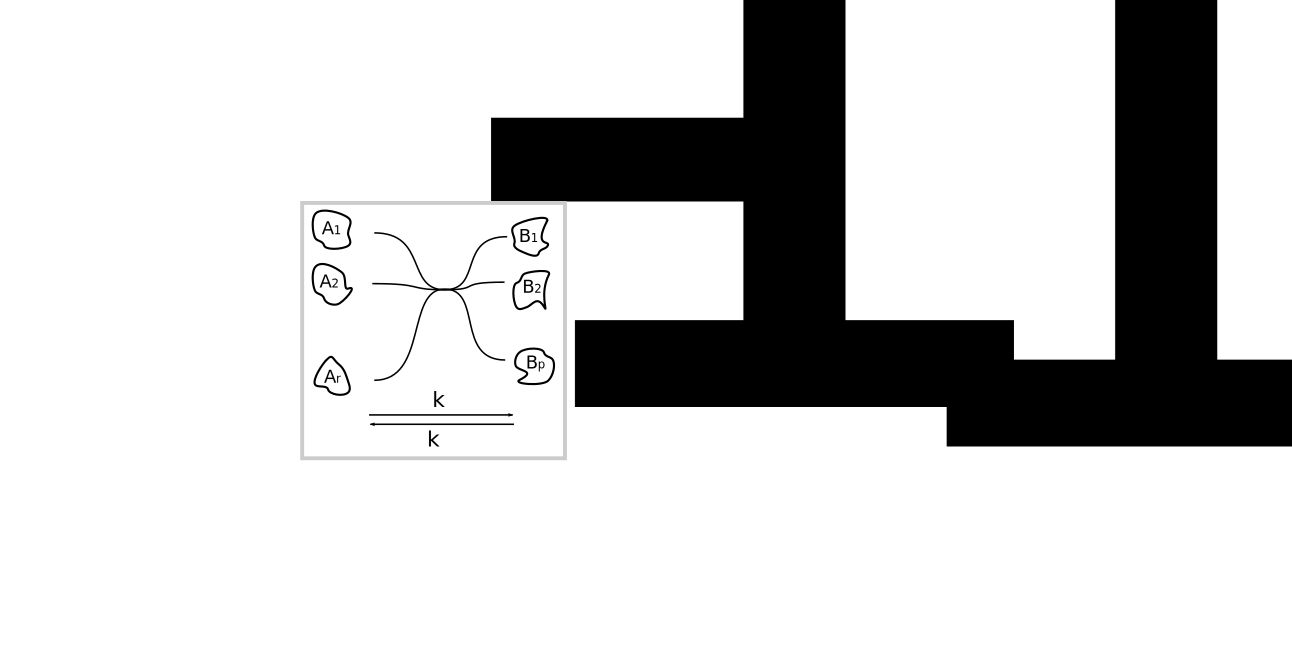
\includegraphics[width=\linewidth]{chemicalreaction}
  \caption{Schematic view of a \texttt{ChemicalReaction}.}
  \label{fig:chemical_reaction}
\end{figure}

\paragraph{Input format}
\begin{verbatim}
ChemicalReaction [<chemical> <stoichiometry>]^{1..n} rates <k_1> <k_-1>
\end{verbatim}

\paragraph{Formula} A \texttt{ChemicalReaction} represents association/dissociation of an arbitrary number of elements~\reffigp{fig:chemical_reaction}. It is defined by
\[
	\reactionRev{a_1 A_1 + a_2 A_2 + ... + a_r A_r}{b_1 B_1 + ... + b_p B_p}{k_1}{k_{-1}}
\]
where
\begin{itemize}
\item $A_i$ and $B_i$ are of type \texttt{FreeChemical}. They can be of type \texttt{BoundChemical} in two cases: (i) a reaction containing a \texttt{BoundChemical} on each side, (ii) an \emph{irreversible} reaction where a \emph{reactant} is a \texttt{BoundChemical} and where there are no bound product. In both cases, the associated stoichiometric coefficient must be 1.
\item $a_i$ and $b_i$ are stoichiometric coefficients.
\item $k_1$ and $k_{-1}$ are rate constants.
\end{itemize}

\paragraph{Action} When the reaction is performed, the number of chemicals involved is changed according to their stoichiometric coefficient. If \texttt{BoundChemical} are involved on each side, the simulator will assume that the bound chemical that is consumed is replaced by the bound chemical on the other side of the equation (\textit{i.e.} it will be bound at the location previously occupied by the precursor). If there is a \texttt{BoundChemical} on the reactant side of an irreversible reaction, the simulator will assume that the reaction describes the unbinding of this bound unit into the cytosol.

\paragraph{Rate} The rates are given by
\[
\lambda_{forward} = k_1 \prod\limits_{i=1}^{r} [A_i]^{a_i}
\]
\[
\lambda_{backward} = k_{-1} \prod\limits_{i=1}^{p} [B_i]^{b_i}
\]

\subsubsection{SequenceBinding}
\paragraph{Input format}

\begin{figure}[!h]
  \centering
  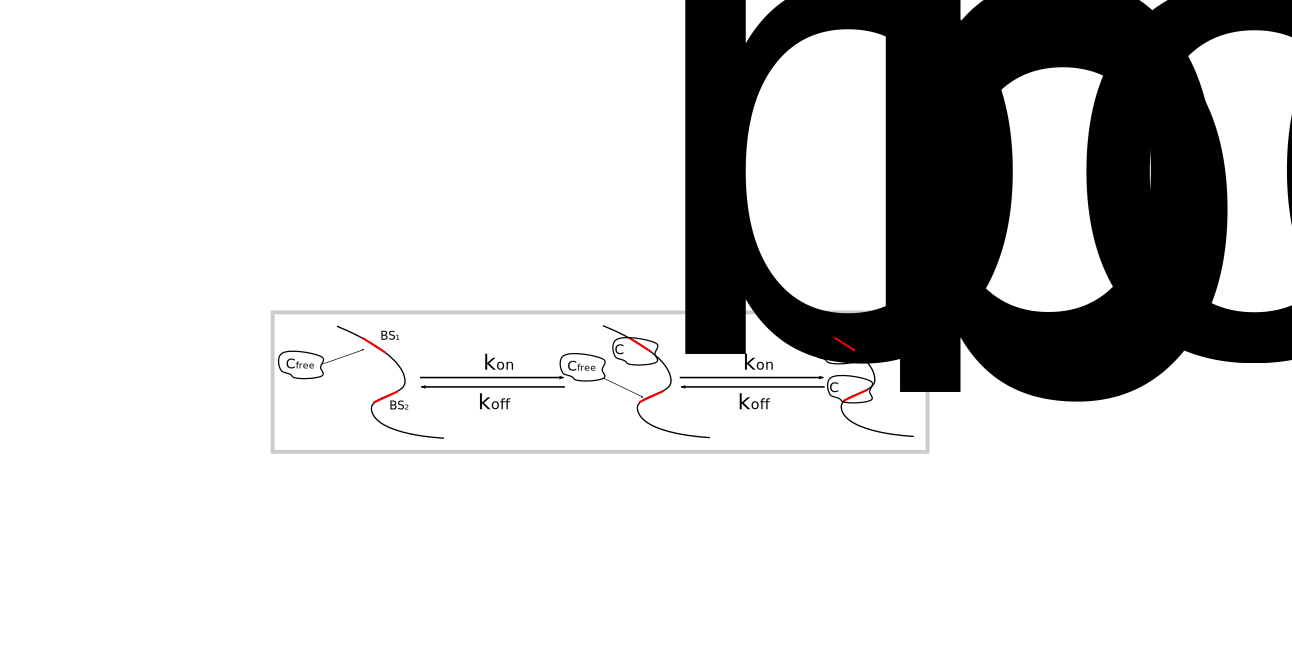
\includegraphics[scale=0.8]{sequencebinding}
  \caption{Schematic view of a \texttt{SequenceBinding}.}
  \label{fig:sequence_binding}
\end{figure}

\begin{verbatim}
SequenceBinding <chemical> <bound form> <binding site family>
\end{verbatim}

\paragraph{Formula} A \texttt{SequenceBinding} represents binding of a free element on a binding site of a sequence~\reffigp{fig:sequence_binding}. It is defined by
\[
\reactionRev{C_{free} + BSF}{C_{bound}}{}{}
\]
where
\begin{itemize}
	\item $C_{free}$ is of type \texttt{FreeChemical}.
	\item $BSF$ is of type \texttt{BindingSiteFamily}.
	\item $C_{bound}$ is of type \texttt{BoundChemical}.
\end{itemize}

\paragraph{Action} When the forward reaction is performed, a random available binding site is drawn from the binding site family (drawing is weighted by affinity). A $C_{free}$ molecule is removed from the pool and a $C_{bound}$ added to the \texttt{ChemicalSequence} bearing the binding site. When the backward reaction is performed, a random molecule of $C_{bound}$ is removed from the pool (and from its sequence) and a $C_{free}$ molecule is added.

\paragraph{Rate} The rates are given by
\[
	\lambda_{forward} = \frac{[C_{free}]}{V_c} \sum_{\text{sites }s \in BSF} (k_{on})_s \times \text{Number of sites $s$ available}
\] 
\[
	\lambda_{backward} = \frac{1}{V_c} \sum_{\text{molecules }m \in C_{bound}} (k_{off})_\text{site on which $m$ is bound}
\]
\begin{itemize}
	\item $(k_{on})_s$ is the association constant of $C_{free}$ with binding site $s$.
	\item $(k_{off})_s$ is the dissociation constant of $C_{bound}$ with binding site $s$.
	\item $V_c$ is the volume of the cell.
\end{itemize}

\subsubsection{Translocation}

\begin{figure}[!h]
  \centering
  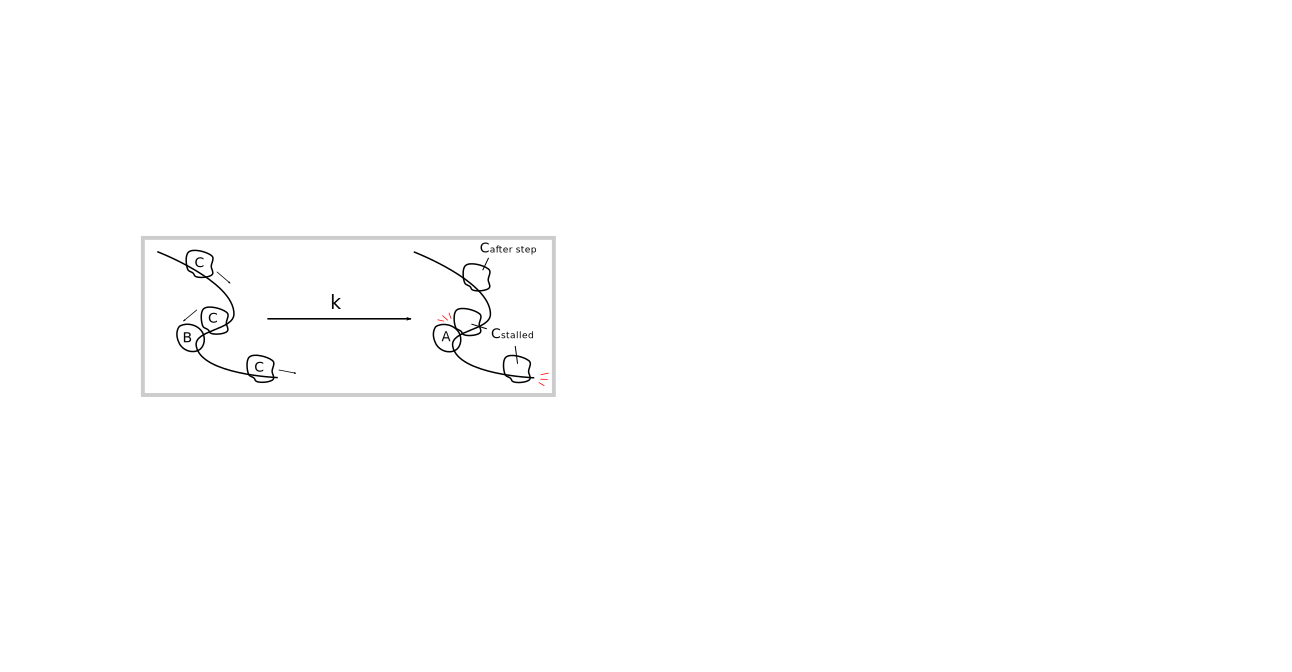
\includegraphics[scale=0.8]{translocation}
  \caption{Schematic view of a \texttt{Translocation}.}
  \label{fig:translocation}
\end{figure}

\paragraph{Input format}
\begin{verbatim}
TerminationSite <family name> <chemical sequence> <start> <end>
Translocation <bound chemical> <form after step> <stalled form> \
  <step size> <rate> [<termination site family>]^{0..n}
\end{verbatim}

\paragraph{Formula} A \texttt{Translocation} represents movement of a bound element along a sequence~\reffigp{fig:translocation}. It is defined by
\[
	\reactionIrr{C}{C_\text{after step}}{k}{}
\]
or
\[
	\reactionIrr{C}{C_\text{stalled form}}{k}{}
\]
where
\begin{itemize}
	\item $C$ is of type \texttt{BoundChemical}.
	\item $C_\text{after step}$ is of type \texttt{BoundChemical}.
	\item $C_\text{stalled form}$ is of type \texttt{BoundChemical}.
	\item $k$ is a rate constant.
\end{itemize}

\paragraph{Action} When the reaction is performed, a random $C$ is chosen. Generally, it is replaced by a $C_\text{after step}$, moved by a step of a given size along the sequence the original $C$ is bound to. If the chemical cannot move because it reached the end of the sequence or it reaches a termination site, it is replaced by $C_\text{stalled form}$.

\paragraph{Rate} The rate is given by
\[
	\lambda = k [C]
\]

\subsubsection{Loading}

\begin{figure}[!h]
  \centering
  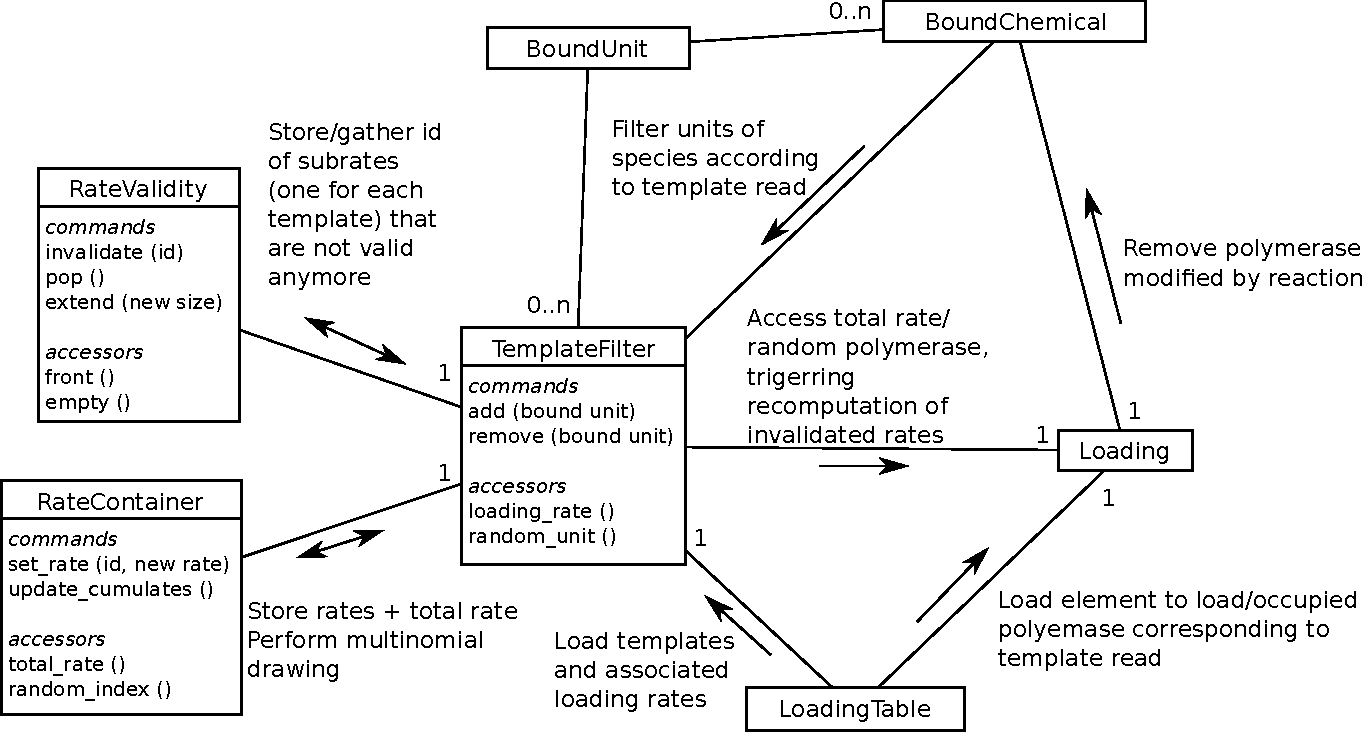
\includegraphics[scale=0.8]{loading}
  \caption{Schematic view of a \texttt{Loading}.}
  \label{fig:loading}
\end{figure}

\paragraph{Input format}
\begin{verbatim}
LoadingTable <name> \
  [<template> <element_to_load> <occupied_polymerase> <rate>,]^{1..n}
ProductLoading <bound chemical> <loading table>
DoubleStrandLoading <bound chemical> <loading table> <stalled form>
\end{verbatim}

\paragraph{Formula} A \texttt{Loading} typically represents loading of elements by a polymerase onto a template sequence~\reffigp{fig:loading}. It is defined by
\[
\reactionIrr{L + E}{LE}{}{}
\]
where
\begin{itemize}
	\item $L$ is of type \texttt{BoundChemical}.
	\item $E$ is an element to load, of type \texttt{FreeChemical}. It is defined in a \texttt{LoadingTable} associated with the reaction.
	\item $LE$ is the occupied form of the loader, of type \texttt{BoundChemical}. It is defined in a \texttt{LoadingTable} associated with the reaction.
\end{itemize}

\paragraph{Action} Each instance of $L$ reads a specific template. Using its \texttt{LoadingTable}, we know which $E$ it tries to load, which $LE$ is yielded if loading occurs and the loading rate associated with the template. When the reaction is performed, a random $L$ is chosen according to loading rates. An element to load $E$ is removed from the pool and $L$ is replaced with $LE$. A \texttt{ProductLoading} assembles loaded elements into a product that will eventually be release in the cytosol (\textit{e.g.} RNA synthesis), while \texttt{DoubleStrandLoading} extends segments along a \texttt{DoubleStrand} (\textit{e.g.} DNA replication). In \texttt{DoubleStrandLoading}, loading may fail because the loader met a previously synthesized segment. In the latter case, it is replaced by a \texttt{BoundChemical} representing its stalled form.

\paragraph{Rate} The rate is given by
\[
\lambda = \sum_{t\in templates} k_t[L_t][E_t]
\]
where
\begin{itemize}
	\item $k_t$ is the loading rate associated with template $t$.
	\item $L_t$ corresponds to loaders $L$ reading template $t$.
	\item $E_t$ is the chemical to load onto template $t$.
\end{itemize}

\subsubsection{DoubleStrandRecruitment}

\begin{figure}[!h]
  \centering
  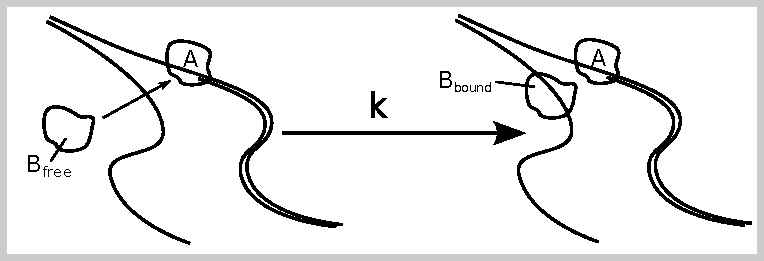
\includegraphics[scale=0.8]{doublestrandrecruitment}
  \caption{Schematic view of a \texttt{DoubleStrandRecruitment}.}
  \label{fig:double_strand_recruitment}
\end{figure}

\paragraph{Input format}
\begin{verbatim}
DoubleStrandRecruitment <BoundChemical> <FreeChemical> <bound form> <rate>
\end{verbatim}

\paragraph{Formula} A \texttt{DoubleStrandRecruitment} typically represents recruitment of a DNA polymerase by the replication fork on the opposite strand~\reffigp{fig:double_strand_rcruitment}. It is defined by
\[
\reactionIrr{A + B_{free}}{A + B_{bound}}{k}{}
\]
where
\begin{itemize}
  \item $A$ is of type \texttt{BoundChemical}
  \item $B_{free}$ is of type \texttt{FreeChemical}
  \item $B_{bound}$ is a \texttt{BoundChemical} representing the bound form of $B_{free}$.
  \item $k$ is a rate constant.
\end{itemize}

\paragraph{Action} When the reaction is performed, a random $A$ is chosen. If $A$ is not bound to a \texttt{DoubleStrand}, the reaction is ignored. If the position opposite to a on the \texttt{DoubleStrand} is already occupied, the reaction is ignored. Else, a $B_{free}$ is bound on the complementary \texttt{ChemicalSequence}, opposite to $A$ as a $B_{bound}$.

\paragraph{Rate} The rate is given by
\[
\lambda = k[A][B_{free}]
\]

\subsubsection{Release}

\begin{figure}[!h]
  \centering
  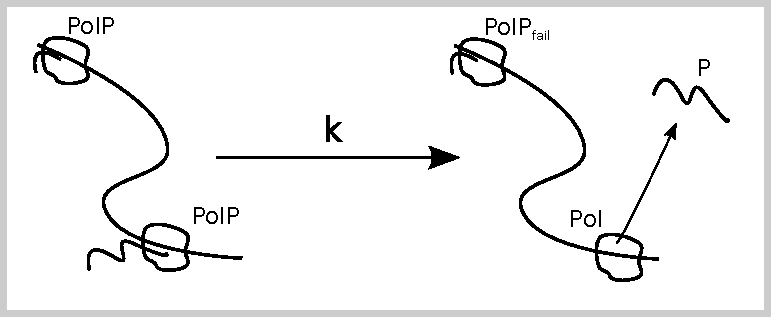
\includegraphics[scale=0.8]{release}
  \caption{Schematic view of a \texttt{Release}.}
  \label{fig:release}
\end{figure}

\paragraph{Input format}
\begin{verbatim}
TransformationTable <name> [<parent_letter> <product_letter>,]^{1..n}
ProductTable <name> <transformation table>
Release <polymerase> <empty_polymerase> <fail_polymerase> \
  <product table> <rate>
\end{verbatim}

\paragraph{Formula} A \texttt{Release} represents release of a product from a polymerase~\reffigp{fig:release}.
\[
	\reactionIrr{PolP}{Pol + P}{k}{}
\]
or 
\[
	\reactionIrr{PolP}{PolP_{fail}}{k}{}
\]
where
\begin{itemize}
	\item $PolP$ is a \texttt{BoundChemical} representing a polymerase-product complex.
	\item $P$ is of type \texttt{ChemicalSequence}. It is a product that is released by $PolP$ defined in a \texttt{ProductTable} associated with reaction.
	\item $Pol$ is a \texttt{BoundChemical} representing an empty polymerase.
	\item $PolP_{fail}$ is a \texttt{BoundChemical} representing the polymerase-product complex in case release failed because $P$ was not a valid product defined in the \texttt{ProductTable} associated with reaction.
	\item $k$ is a rate constant.
\end{itemize}

\paragraph{Action} When the reaction is performed, a random $PolP$ is chosen. A \texttt{ProductTable} uses its binding and current position to determine what product $P$ it has synthesized. If $P$ is defined in the product table, it is released in the cytosol and $PolP$ is replaced by an empty version of the polymerase $Pol$. If there is no $P$ corresponding to current $PolP$ position, the simulator assumes that $PolP$ has not reached its actual terminator and it is replaced by $PolP_{fail}$ to enable other treatments (\textit{e.g.} abnormal termination or continuing synthesis).

\paragraph{Rate} The rate is given by
\[
\lambda = k[PolP]
\]

\subsubsection{Degradation}

\begin{figure}[!h]
  \centering
  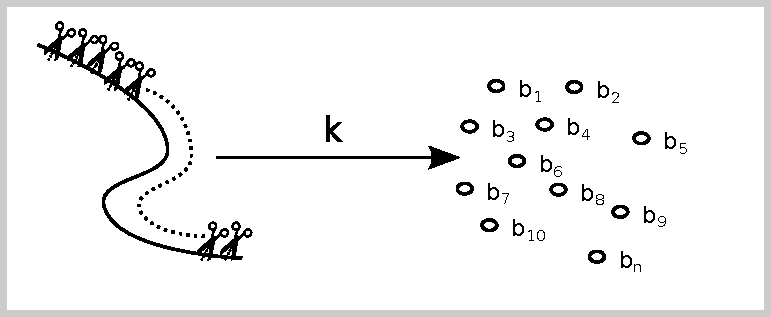
\includegraphics[scale=0.8]{degradation}
  \caption{Schematic view of degradation reaction.}
  \label{fig:degradation}
\end{figure}

\paragraph{Input format}
\begin{verbatim}
CompositionTable <name> [<letter> [<chemical composing letter>]^{1..m}]^{1..n}
Degradation <chemical sequence> <composition table> <rate>	
\end{verbatim}

\paragraph{Formula} A \texttt{Degradation} represents decomposition of a sequence into base components~\reffigp{fig:degradation}. It is defined by
\[
\reactionIrr{CS}{b_1 + b_2 + ... + b_N}{k}{}
\]
where
\begin{itemize}
	\item $CS$ is of type \texttt{ChemicalSequence}.
	\item $b_i$ are of type \texttt{FreeChemical}. They are found in a \texttt{CompositionTable} specified in the reaction.
	\item $k$ is the degradation constant.
\end{itemize}

\paragraph{Action} When the reaction is performed, a $CS$ is removed from the pool. A \texttt{CompositionTable} is specified along the reaction. It allows base-by-base conversion of the sequence of $CS$ into components yielded by degradation. The pools of base components is updated accordingly. In the simulator, a degradation reaction is effectively implemented as a \texttt{ChemicalReaction}.

\paragraph{Rate} The rate is given by
\[
\lambda = k [CS]
\]
